\documentclass{article}
\usepackage[utf8]{inputenc}
\usepackage{graphicx} 
\usepackage{natbib} 
\usepackage[portuguese]{babel} %Pra deixar "References" em português.


\title{Projeto LATEX}
\author{Guimel Filipe Gomes Cavalcante}
\date{Setembro 2022}

\begin{document}

\maketitle

\begin{figure} [h!]
    \centering
    
\includegraphics[scale = 0.5]{cin.png}
\end{figure}
\begin{center}
    {\LARGE Informática e sociedade}
\end{center}


\section{Introdução}
\paragraph{} A disciplina de Informática e Sociedade aborda o impacto social de novas tecnologias na história, desde mudanças sociológicas causadas pela informática até a percepção da sociedade sobre essas mudanças. Usando conceitos gerais de sociologia para discutir ética e direito sobre temas como cibercrimes, propriedade intelectual, segurança de dados e privacidade através de estudos de casos.

\section{Relevância}
\paragraph{} "Não se pode estudar os efeitos da informática e das tecnologias sobre os indivíduos e a cultura sem recorrer-se às mudanças diárias." \citep{Manuel} A partir disso, é possível dizer que a revolução das tecnologias da informação atua remodelando as formas de organização social. Uma vez que a informação e consequentemente acesso a novas tecnologias tornam-se importantes ferramentas na geração de riqueza e exercício de poder.
\paragraph{} Essas discussões podem trazer benefícios como por exemplo:
\begin{itemize}
    \item Abrangência de movimentos sociais e culturais.
    \item Proporcionar uma melhor qualidade de vida para sociedade. 
    \item Criação e padronização de leis para crimes digitais.
    
\end{itemize}

\section{Relação com outras disciplinas}
\paragraph{} "O estudo do impacto da informática na sociedade pode ser associado à muitas outras áreas do conhecimento"\citep{Simon} já que a interação ser humano e máquina se mostra cada vez mais presente como podemos ver em outras disciplinas ofertados no Centro de Informática da Univesidade Federal de Pernambuco.

\paragraph{} A disciplina IF681 - Interface usuário-máquina é um ótimo exemplo de como aplicar a percepção da sociedade sobre a tecnologia para gerar uma comunicação mais fluída na criação de interfaces.
\begin{figure}[h!]
    \centering
    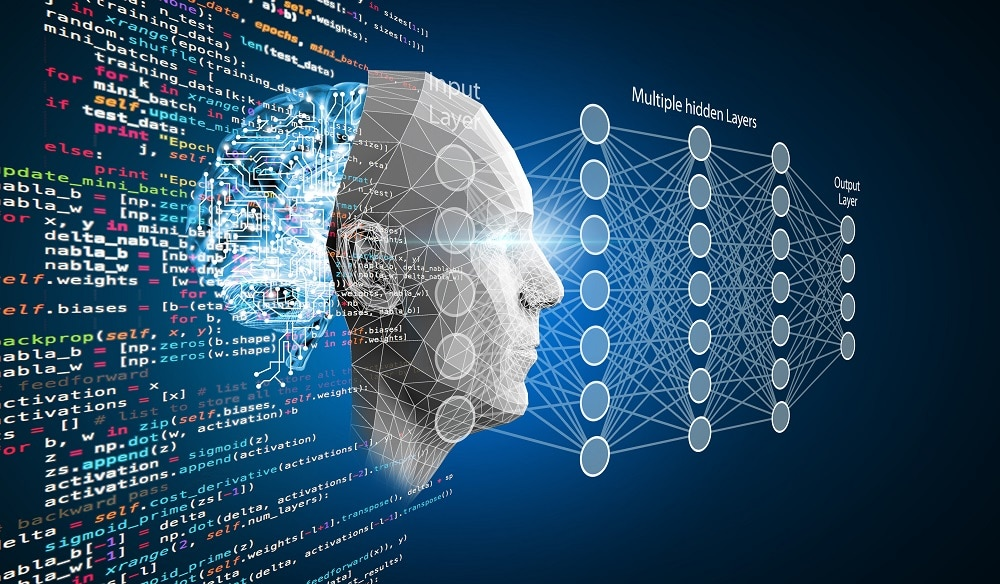
\includegraphics[scale = 0.17]{interface.jpg}
    \caption{Imagem ilustrando interface usuário-máquina.}\citep{interface}
    
\end{figure}

\paragraph{} A disciplina IF699 - Aprendizagem de máquina é outra área com grande crescimento no uso de dados gerados a partir da interação entre pessoas e máquinas para criar parâmetros na criação de inteligências artificiais.


\bibliographystyle{abbrv}
\bibliography{referências}


\end{document}
